\subsection{Platform-as-a-Service (PaaS)}
PaaS clouds host web-accessible (HTTP/S) applications, to which they provide 
high levels of scalability, availability, and sandboxed execution. 
PaaS clouds provide scalability by automatically allocating resources 
for applications on the fly (auto scaling), and provide availability through
the execution of multiple instances of the application and/or the PaaS
services they employ for their functionality.
PaaS clouds provide a high level of abstraction to the application developer that effectively hides
all the infra\-structure-level details such as physical resource allocation (CPU, memory, disk etc), operating
system,
and network configuration. This enables application developers to focus solely on the programming
aspects of their applications, without having to be concerned about deployment issues. 
Consequently, viable PaaS technologies as well as
PaaS-hosted applications have been increasing rapidly in number~\cite{paas-growth}.
But due to the high level of abstraction, performance monitoring and root cause analysis
is particularly challenging in PaaS clouds. Due to this reason, and the large number of 
PaaS applications available for testing, we design Roots APM to operate within PaaS
clouds.

\begin{figure}
\centering
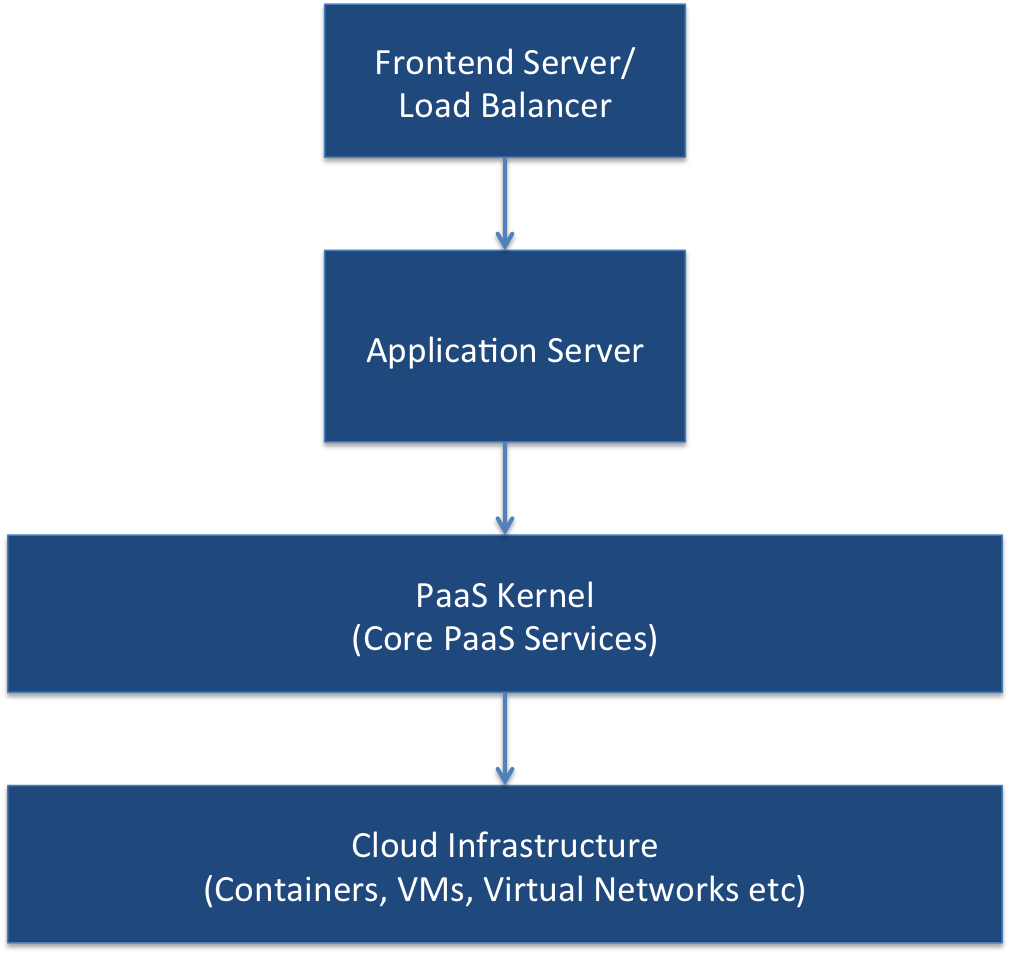
\includegraphics[scale=0.5]{paas_architecture}
\caption{PaaS system organization.}
\label{fig:paas_architecture}
\end{figure}

Figure~\ref{fig:paas_architecture} shows the key layers of a typical PaaS cloud. Arrows indicate
the flow of data and control in response to application requests.

At the lowest level of a PaaS cloud is an infrastructure that consists of the necessary compute, storage
and networking resources. How this infrastructure is set up may vary from a simple cluster of physical 
machines to a comprehensive Infrastructure-as-a-Service (IaaS) solution. In large scale PaaS clouds,
this layer typically consists of many virtual machines and/or containers with the ability to acquire more
resources on the fly.

On top of the infrastructure layer lies the PaaS kernel. This is a collection of managed, scalable
services that high-level application developers can compose into their applications. The provided services
may include database services, caching services, queuing services and much more. Some PaaS clouds
provide a managed set of APIs (an SDK) for the application developer to access these fundamental services. 
In that case all interactions between the applications and the PaaS kernel must take place through
the cloud provider specified APIs (e.g. Google App Engine). 

One level above the PaaS kernel we find the application servers that are used to deploy and run
applications. Application servers provide the necessary integration (linkage) between application code and the
underlying PaaS kernel, while sandboxing application code for secure, multi-tenant operation. On top
of the application servers layer resides the fronted and load balancing layer. This layer is responsible
for receiving all application requests, filtering them and routing them to an appropriate application
server instance for further execution. As the fronted server, it is the entry point for PaaS-deployed
applications for all application clients.

Each of the above layers can span multiple processes, running over multiple physical or virtual
machines. Therefore the execution of a single application request typically involves cooperation
of multiple distributed processes and/or machines. In order to perform comprehensive monitoring
and root cause analysis, we need to be able to monitor each of the above layers along with their
enclosed components. Further we need to be able to trace the flow of data and control
across different layers and components.

\subsection{Cloud-hosted Web Applications}
Our work concentrate on the web applications deployed in PaaS clouds. An application of this nature
exposes one or more web application programming interfaces (web APIs) through which clients can
interact with it. The web APIs accept HTTP/S requests sent by remote clients, and respond with
machine readable responses (e.g. HTML, JSON, XML, Protocol Buffers). This type of applications tend to be highly
interactive, and clients typically have tight expectations on the application response time. The PaaS 
cloud on which an application is running on may impose additional constraints on the application
response time for scalability reasons. For example Google App Engine requires that no application
request takes more than 60 seconds to execute.

PaaS-hosted web applications also rely on the various PaaS kernel services offered by the underlying
cloud platform. By offloading common application functionality such as data storage, caching,
user management, and security to a set of managed cloud services, application developers
can greatly reduce the amount of code they have to write. It also eliminates the need to install, run and
manage many other support applications that would otherwise be necessary (e.g. a database server, 
a message broker etc.). In other words, when developing applications for a PaaS environment, the
developer only need to think about getting his/her application code to work. All other deployment
and utility services are provisioned by the PaaS cloud. 

The downside of this approach is that application developers no longer have full runtime visibility
into the application execution. Since most of the application functionality is provided by a set 
of PaaS kernel services that are in cloud provider's domain, the application
developer does not have total control over application performance. If the application 
response time becomes too slow, the application developer is not in a position to determine
where in the entire cloud platform, the performance bottleneck is. One way to circumvent this 
limitation is to instrument application code, and continuously monitor the time taken by various
parts of the application. But this is tedious on the part of the application developer, and
the additional code instrumentation slows down the entire application.

\subsection{Performance Anomalies}